\documentclass{beamer}
\usepackage{amsmath,amsxtra,amssymb,latexsym, amscd,amsthm}
\usepackage{indentfirst}
\usepackage[mathscr]{eucal}
\usepackage[utf8]{vietnam}
\usepackage{indentfirst}
\usepackage{array}
\usepackage{setspace}
\usepackage{graphicx}
\usepackage{xhfill}
\usepackage[left=2cm,right=2cm,top=2cm,bottom=2cm]{geometry}

\begin{document}
%Cover
\begin{frame}
    \begin{center}
    \fontsize{10pt}{20pt}\selectfont
    \textsc{TỔNG LIÊN ĐOÀN LAO ĐỘNG VIỆT NAM\\}
    \textbf{TRƯỜNG ĐẠI HỌC TÔN DỨC THẮNG\\}
    \textbf{KHOA CÔNG NGHỆ THÔNG TIN\\}
    
        \begin{figure}[htp]
            \centering
           
\includegraphics[scale = 0.5]{2.jpg}
        \end{figure}
    
    \fontsize{12}{20}\selectfont\textbf{ĐỒ ÁN CUỐI KHÓA:\\}
    \fontsize{12}{20}\selectfont\textbf{MÔN PHÁT TRIỂN HỆ THỐNG THÔNG TIN DOANH NGHIỆP\\}
    \fontsize{14}{20}\selectfont\textsc{PHÂN TÍCH VÀ THIẾT KẾ\\ HỆ THỐNG CỬA HÀNG BÁN DỤNG CỤ THỂ THAO SALOMON \\}
    \end{center}
\end{frame}
%Mục lục
\begin{frame}[plain]
    \frametitle{Mục lục} 
    \fontsize{10}{20}\selectfont\textbf{Chương 1: Đặc tả tóm tắt hệ thống Salomon}\\
    \fontsize{9}{20}\selectfont\textsc{Chương 1.1: Thanh toán}\\
    \fontsize{9}{20}\selectfont\textsc{Chương 1.2: Quản lý hóa đơn}\\
    \fontsize{9}{20}\selectfont\textsc{Chương 1.3: Quản lý kho}\\
    \fontsize{9}{20}\selectfont\textsc{Chương 1.4: Bảo hành}\\[0.2cm]
    \fontsize{10}{20}\selectfont\textbf{Chương 2: Đặc tả chi tiết}\\
    \fontsize{9}{20}\selectfont\textsc{Chương 2.1: Nghiệp vụ thanh toán} \\
    \fontsize{9}{20}\selectfont\textsc{Chương 2.2: Quy trình quản lý hóa đơn} \\
    \fontsize{9}{20}\selectfont\textsc{Chương 2.3: Quy trình quản lý kho}\\[0.2cm]
    
\end{frame}


%Chương1

\begin{frame}
    \frametitle{Chương 1: Đặc tả tóm tắt hệ thống Salomon}
     Cửa hàng gồm có 3 chức vụ sau: Quản lý tổng, Nhân viên bán hàng,Nhân viên kho
    \begin{itemize}
        \item Đứng đầu là quản lý
        \item Nhân viên viên bán hàng có trách nhiệm ở cửa hàng
        \item Nhân viên kho quản lý kho ở từng chi nhánh sau đó báo lại cho quản lý
    \end{itemize}
\end{frame}
%1.1 - Quản lý
\begin{frame}{Chương 1.1 : Thanh toán}
    Nhân viên thanh toán sẽ tạo hóa đơn và quét mã sản phẩm (Mã Barcode) \\
    
    Nhân viên thông báo số tiền thanh toán và cách thức thanh toán cho khách hàng \\
    
    Có 3 cách thanh toán:
    \begin{itemize}
        \item Tiền mặt
        \item Quẹt thẻ
        \item Chuyển khoảng
    \end{itemize}\\
    Nếu khách hàng đặt hàng online thì khách hàng sẽ chọn thanh toán sau khi nhận hàng
\end{frame}
\begin{frame}{Chương 1.1: Thanh toán}
    Sau khi thanh toán, nhân viên cần lưu thông tin của khách hàng:\\
    \begin{itemize}
        \item Tên
        \item Số điện thoại
    \end{itemize}\\
    Khi hoàn thành việc thanh toán và nhập thông tin khác hàng, nhân viêc kết thúc hóa đơn bằng việc "Done bill"\\
    Khi đó thông tin khách hàng, thông tin hóa đơn, số lượng của sản phẩm được cấp nhật trên hệ thống tổng.
\end{frame}

%Chương 1.2
\begin{frame}{Chương 1.2: Quản lí hóa đơn}
    Quản lý hóa đơn dùng để lưu trữ tất cả các hóa đơn được thanh toán tại cả 2 chi nhánh của cửa hàng  \\
    Được truy cập bởi quản lý tổng. \\
    Hệ thống quản lý hóa đơn chỉ được truy cập bởi quản lý cửa hàng.\\
    Quản lý cửa hàng có thể thực hiện cách thao tác
        \begin{itemize}
            \item chỉnh sửa thay đổi
            \item xóa hóa đơn mới trong hệ thong quản lý hóa đơn
            \item thống kê lại các hóa đơn của tháng
        \end{itemize}
\end{frame}
%Chương 1.3
\begin{frame}{Chương 1.3: Quản lí kho}
    Cửa hàng hiện có 3 kho đó là kho tổng và kho tại cửa hàng Tp.HCM và cửa hàng tại Hà Nội.\\
    
    Nhân viên kho phụ trách gồm các công việc tìm kiếm và kiểm tra số lượng các sản phẩm trong kho, xuất kho .nhập kho\\
\end{frame}
\begin{frame}{Chương 1.3: Quản lí kho - Tìm Kiếm sản phẩm}
    Nhân viên có thể kiểm tra và tìm kiếm lọc các sản phẩm trong kho theo các thông tin của sản phẩm:

    \begin{itemize}
        \item Kho
        \item Mã sản phẩm
        \item Tên sản phẩm
        \item Size
        \item Số lượng 
    \end{itemize}\\
    Sau khi nhập các thông tin của sản phẩm cần tìm kiếm, trang quản lý kho sẽ hiển thị danh sách các sản phẩm theo thông tin được tìm kiếm
\end{frame}
\begin{frame}{Chương 1.3: Quản lí kho - Xuất kho}
   Xuất kho là khi muốn xuất các sản phẩm từ kho này về kho khác. Xuất kho thực hiên theo trình tự
   \begin{itemize}
    
        \item Khi xuất kho, nhân viên kho sẽ tạo danh sách xuất kho và chọn kho được xuất đi
        \item Sau khi tạo danh sách xuất kho, nhân viên kho sẽ thực hiện 
        \item nhập lần lượt thông tin các sản phẩm được xuất đi
        \item Nhân viên thực hiện in và chốt danh sách nhập kho. 
        \item Khi chốt danh sách, trang quản lý kho sẽ gửi thông điệp thực hiện cập nhật trừ đi số lượng sản phẩm được xuất đi trong kho đó
   \end{itemize}
\end{frame}
\begin{frame}{Chương 1.3: Quản lí kho - Nhập kho}
    Nhập kho gồm có 3 ngữ cảnh là 
    \begin{enumerate}
        \item Sản phẩm nhập từ hãng về
        \item Sản phẩm được nhập từ kho khác về
        \item Sản phẩm khách đổi trả
    \end{enumerate}
    Khi nhập kho, nhân viên kho thực hiện
    \begin{itemize}
        \item Tạo danh sách nhập kho 
        \item Chọn kho được nhập
        \item Nhập lần lượt thông tin các sản phẩm được nhập về. 
        \item Nhân viên thực hiện in và lưu danh sách nhập kho
    \end{itemize}
\end{frame}
\begin{frame}{Chương 1.4: Bảo hành}
    \begin{itemize}
        \item [$\nabla$]Sản phẩm sẽ được kiểm tra lỗi sản phẩm theo quy định và kiểm tra sản phẩm còn nằm trong chương trình bảo hành hay không 
     
    \item [$\nabla$] Nếu sản phẩm được mua ở cửa hàng và nằm trong điều kiện bảo hành sản phẩm, thực hiện tạo hóa đơn nhận bảo hành sản phẩm và nhập thông tin sản phẩm được nhận bảo hành, in hóa đơn nhận bảo hành cho khách
     
    \item [$\nabla$] Nhân viên kho sẽ thực hiện bảo hành sản phẩm cho khách. Hóa đơn bảo hành sẽ có 2 chế độ: Đang bảo hành và Đã bảo hành
    \end{itemize}
\end{frame}
\begin{frame}{Sơ đồ}
    \begin{figure}[htp]
        \centering
        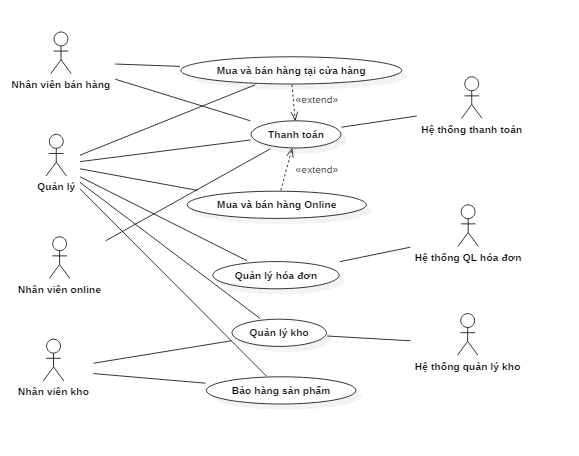
\includegraphics[scale = 0.7]{3.png}
    \end{figure}
\end{frame}
%Chương 2
\begin{frame}
    \fontsize{20}{20}\selectfont\textbf{Chương 2:Đặc tả chi tiết}
\end{frame}
%Chương 2.1
\begin{frame}{Chương 2.1: Nghiệp vụ thanh toán}
    Sau khi hoàn tất các bước chọn sản phẩm cũng như kiểm tra đầy đủ các thông tin cần thiết của khách hàng\\
    
    Nhân viên thanh toán sẽ phải tạo một trang thanh toán trên hệ thống thanh toán hóa đơn của shop
    
    Trang thanh toán sẽ bao gồm những thông tin khách hàng đồng thời cũng cung cấp những chi tiết của đơn hàng bao gồm : 

        \begin{itemize}
            \item Tên của hàng
            \item Bảng danh sách sản phẩm
            \item Tổng hóa đơn
            \item Khách thanh toán: Tiền mặt, Card. Thanh toán khi nhận hàng. chuyển khoảng
            \item Tiền thối
            \item Thông tin khách hàng: Họ Tên, Số điện thoại
            \item Ghi chú
            \item In hóa đơn
            \item Hoàn tất hóa đơn
        \end{itemize}
\end{frame}
\begin{frame}{Chương 2.1: Nghiệp vụ thanh toán}

    \begin{itemize}
        \item [$\nabla$] Nhân viên thực hiện nhập thông tin sản phẩm thông qua barcode của sản phẩm\\
        \item [$\nabla$] Sau khi nhập thông tin sản phẩm ,trang thanh toán sẽ hiện nút “In bill” và cho phép nhân viên in bill cho khách kiểm tra và trang thanh toán sẽ cho phép nhập thông tin khách hàng\\
        \item [$\nabla$]Khi khách thanh toán nhân viên có thể chọn một hoặc nhiều phương thức gồm có 4 phương thức: tiền mặt, Thẻ, Chuyển khoản, Thanh toán khi nhận hàng ( dành cho đặt hàng online)\\
          Trang thanh toán sẽ hiện ra khung nhập số tiền cho phương thức thanh toán đó sau khi nhập đủ số tiền khách hàng phải thanh toán thì hệ thống sẽ hiện ra “ Done Bill” . 
        \item [$\nabla$] .Trang thanh toán thực hiệ in thêm một hóa đơn đã thanh toán. Hóa đơn đó sẽ không được thay đổi hay cập nhật nữa.Trang thanh toán được đặt lại(reset)
                                        
    \end{itemize}
\end{frame}
\begin{frame}{Chương 2.1: Nghiệp vụ thanh toán}
    \begin{figure}[htp]
        \centering
        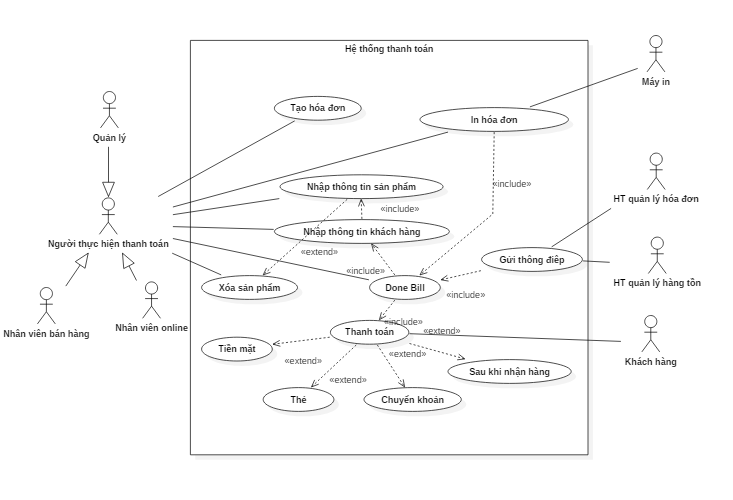
\includegraphics[scale=0.5]{4.png}
    \end{figure}
\end{frame}
\begin{frame}{Biểu đồ thanh toán}
        \begin{figure}
    \centering
    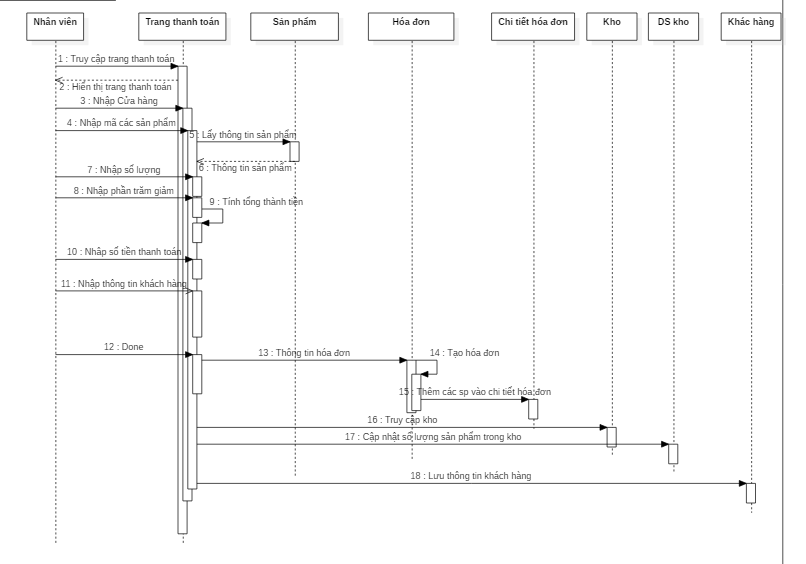
\includegraphics[scale = 0.5]{8.png}\\
    \fontsize{12}{20}\selectfont\caption{Biểu đồ Squence thanh toán}
    
\end{figure}
\end{frame}


%Chương 2.2
\begin{frame}{Chương 2.2: Qui trình quản lí hóa đơn}
    Hệ thống quản lý hóa đơn cung cấp dịch vụ cho đối tượng : Người quản lý\\
    Hệ thống quản lý hóa đơn chỉ được truy cập và điều hàng bởi người quản lý cửa hàng\\
    Hệ thống hóa đơn chỉ được quản lý bởi người quản lý chủ cửa hàng  vì lí do bảo vệ thông tin khách hàng\\
    
    Những thông tin gồm có trên một hóa đơn được quản lý bởi hệ thống bao gồm:
    \begin{itemize}
        \item Tên cửa hàng (Chi nhánh Nguyễn Trãi, TPHCM; chi nhánh Hà Nội)
        \item Thời gian
        \item ID Khách hàng (Số điện thoại khách hàng)
        \item Danh sách các sản phẩm
        \item Số tiền thanh toán(Tiền mặt, Thanh toán khi nhận hàng, Chuyển khoản)
    \end{itemize}
\end{frame}
\begin{frame}{Chương 2.2:Qui trình quản lí hóa đơn}
    \begin{itemize}
        \item[$\nabla$]Sau khi qua quy trình thanh toán và tạo hóa đơn do nhân viên cửa hàng thực hiện\\
        \item[$\nabla$]Mỗi khi nhân viên nhấn nút  “Done bill  “trên trang thanh toán Hệ thống sẽ tạo một hóa đơn dựa vào những thông tin cần thiết\\
        \item[$\nabla$]Mỗi hóa đơn sẽ có được cấp một mã hóa đơn riêng và thêm vào danh sách hóa đơn trên hệ thống và hệ cơ sở dũ liệu. \\
        \item[$\nabla$]Khi một hóa đơn đã được chốt trên trang thanh toán, đã được “ Done” thì hóa đơn đó không thể được thay đổi trên trang thanh toán. Nhưng hóa đơn có thể được quản lý thay đổi hoặc cập nhật thông tin cho hóa đơn.\\
    \end{itemize}
\end{frame}
\begin{frame}{Chương 2.2:Qui trình quản lí hóa đơn}
    Quản lý có thể thay đổi thông tin của hóa đơn trên hệ thống. Sẽ có 2 ngữ cảnh khi thay đổi thông tin hóa đơn trên hệ thống. :
    
    \begin{itemize}
        \item Thay đổi thông tín sản phẩm(số lượng, phần trăm,ghi chú): Thêm hoặc xóa sản phẩm trong đơn hàng, chỉnh sửa phần trăm giảm giá hoặc ghi chú của từng sản phẩm
        \item Thay đổi thông tin khách hagf: thay đôi tên hoặc ID khách hàng
    \end{itemize}
    Sau khi hoàn tất việc thay đổi thông tin, Quản lý sẽ chốt hóa đơn, Nếu thông tin số lượng sản phẩm của các hóa đơn được thay đổi, hệ thống quản lý hóa đơn sẽ gửi một thông điệp thông báo đến hệ thống quản lý hàng tồn cập nhật lại các số lượng các sản phẩm xuất kho cửa hàng (đã bán).
\end{frame}
\begin{frame}{Chương 2.2: Qui trình quản lí hóa đơn}
    \begin{figure}
        \centering
        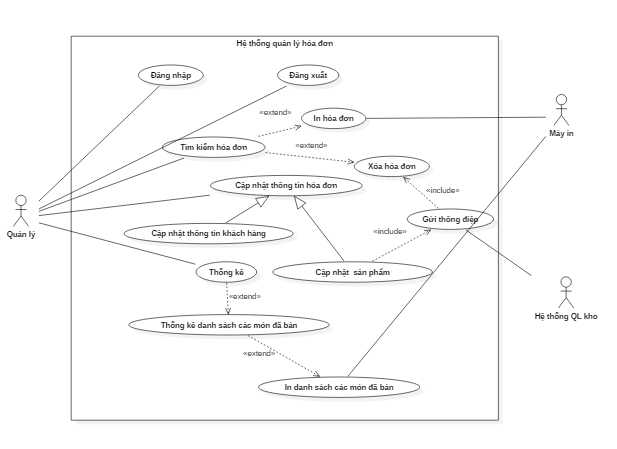
\includegraphics[scale = 0.6]{5.png}
    \end{figure}
\end{frame}
\begin{frame}{Sơ đồ}
    \begin{figure}
    \centering
    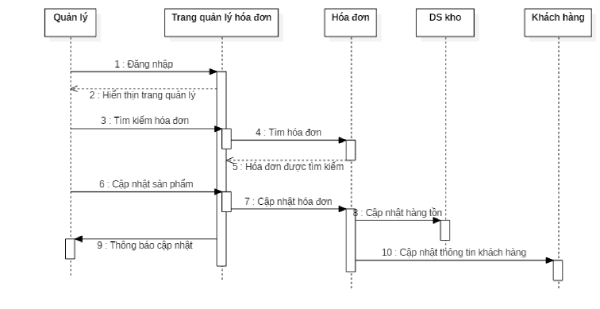
\includegraphics[scale = 0.6]{9.png}

\end{figure}
\end{frame}

%Chương 2.3
\begin{frame}{Chương 2.3: Qui trình quản lí kho}
    Quản lý kho hàng tồn hệ thống sẽ tập trung vào việc xuất, nhập kho của các sản phẩm và thông qua việc đối chiếu các danh sách nhập, xuất để đảm bảo tính xác thực và tin cậy của kho\\
    
    Trang quản lý kho sẽ có những chức năng chính:
    \begin{itemize}
        \item Tìm kiếm 
        \item Kiểm tra sản phẩm trong kho
        \item Tạo danh sách nhập kho/ xuất kho
    \end{itemize}
\end{frame}

\begin{frame}{Chương 2.3: Qui trình quản lí kho}
    \begin{figure}
        \centering
        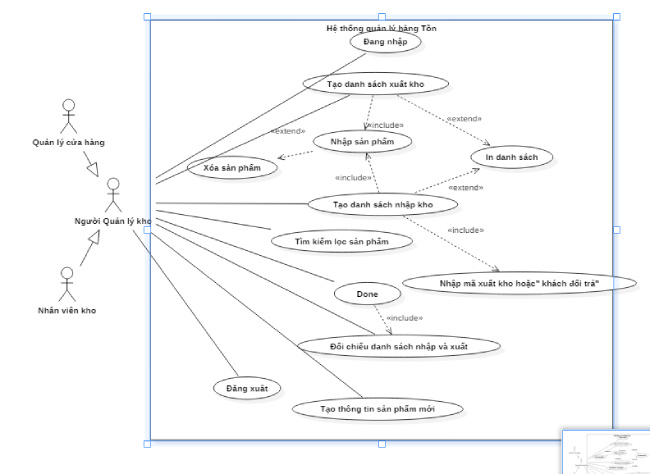
\includegraphics[scale = 0.6]{6.png}
    \end{figure}
\end{frame}
\begin{frame}{CHương 2.3: Qui trình quản lí kho - Tìm kiếm}
    \begin{itemize}
        \item[$\nabla$]Nhân viên chọn kho cần tìm sản phẩm trong trnag quản lí kho
        \item[$\nabla$]Hệ thống sẽ hieencr thị danh sách sản phẩm và bộ lọc tìm kiếm bao gồm những thông tin sau:
            \begin{itemize}
                \item Mã sản phẩm
                \item Tên sản phẩm
                \item Size
                \item Loại
                \item Giá sản phẩm
                \item Số lượng
            \end{itemize}\\
        \item[$\nabla$]Hệ thống sẽ trả về danh sách sản phẩm với các thông tin được tìm kiếm \\
    \end{itemize}
\end{frame}
\begin{frame}{Chương 2.3: Qui trình quản lí kho-Tạo danh sách xuất kho}
    Nhân viên kho sẽ thực hiện tạo danh sách xuất kho khi muốn xuất sản phẩm\\
    nhân viên kho sẽ thực hiện nhập thông tin sản phẩm thông qua  Mã Sản phẩm\\
    Trang quản lý sẽ tự động điền những thông tin của sản phẩm dựa trên mã sản phẩm\\
    Danh sách sẽ hiển thị những thông tin gồm: 
        \begin{itemize}
            \item Ngày nhập kho
            \item Kho xuất đi
            \item Danh sách sản phẩm xuất kho
            \item Tổng số sản phẩm
        \end{itemize}\\
    Sau khi nhập đầy đủ các sản phẩm và thông tin sản phẩm nhập kho, nhân viên kho sẽ thực hiện chốt danh sách ( Done)
\end{frame}

\begin{frame}{Sơ đồ Xuất kho}
    \begin{figure}
        \centering
        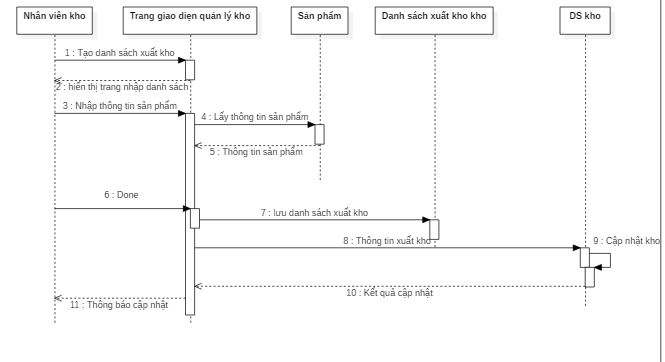
\includegraphics[scale = 0.5]{20.png}
        \caption{Biểu đồ Squence xuất kho}
    \end{figure}
\end{frame}

\begin{frame}{Sơ đồ Xuất kho}
    \begin{figure}
        \centering
        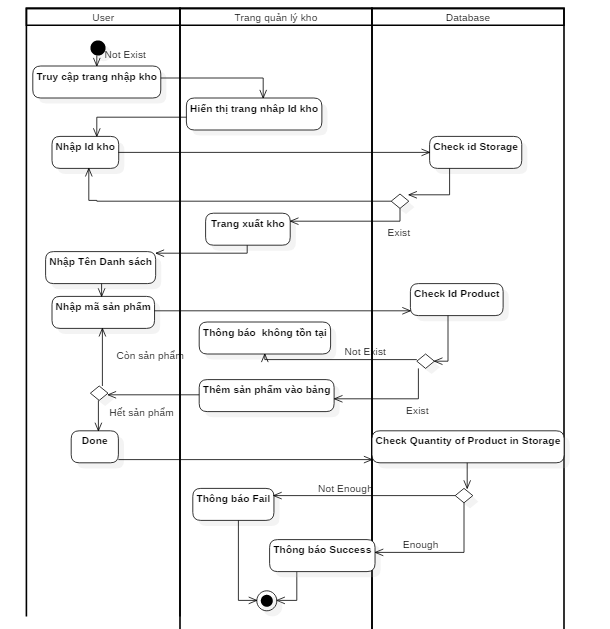
\includegraphics[scale = 0.4]{32.png}
        \caption{Biểu đồ activity xuất kho}
    \end{figure}
\end{frame}

\begin{frame}{Chương 2.3: Qui tình quản lí kho-Tạo danh sách nhập kho}
    Nhập kho sẽ gồm có 3 ngữ cảnh:
    \begin{itemize}
        \item Nhập kho các sản phẩm từ kho tổng về kho cửa hàng hoặc từ cửa hàng về cửa hàng\\
        \item Nhập kho các sản phẩm từ hãng về kho tổng
        \item Khách hàng đổi trả sản phẩm
    \end{itemize}\\
    Sau khi tạo danh sách, nhân viên kho sẽ thực hiện nhập thông tin sản phẩm thông qua Mã sản phẩm\\
    Danh sách sẽ hiển thị những thông tin gồm: 
        \begin{enumerate}
            \item Ngày xuất kho
            \item Kho Xuất đi
            \item Mã sản phẩm
            \item Category:
                \begin{itemize}
                    \item Giày dép
                    \item Quần áo
                    \item Phụ kiện
                \end{itemize}
            \item Size
            \item Số lượng
            \item Tổng sản phẩm
        \end{enumerate}
\end{frame}
\begin{frame}{Chương 2.3: Qui tình quản lí kho-Tạo danh sách nhập kho}
    Sau khi nhập đầy đủ các sản phẩm và thông tin sản phẩm trong danh sách nhân viên sẽ thực hiện chốt danh sách và danh sách khôn g thể bị thay đổi. 
        \begin{enumerate}
            \item 	Nếu ngữ cảnh (1), nhân viên sẽ chọn mục “ nhập từ hãng về” và  mục ghi chú của danh sách nhập kho là “Danh sách sản phẩm được nhập từ hãng về ngày ../ .. /  .. “ 
            \item 	Nếu ngữ cảnh (2), nhân viên sẽ chọn mục “ Nhập từ kho khác”, và thực hiện nhập mã danh sách xuất kho muốn đối chiếu. trang quản lý sẽ gửi thông điệp yêu cầu đối chiếu danh sách nhập kho vói danh sách xuất kho với mã tương ứng với mã danh sách xuất kho được nhập vào. Mục ghi chú của danh sách nhập kho sẽ có nội dung “  Danh sách sản phẩm được nhập từ kho .. (Mã danh sách xuất kho) ngày ../  ../  .. “.
            \item 	Nếu ngữ cảnh (3), nhân viên sẽ chọn mục “ Khách đổi trả”, Mục ghi chú của danh sách nhập kho sẽ là “ 
            Khách đổi trả ngày ../ ../ ..”
        \end{enumerate}
\end{frame}
\begin{frame}{Chương 2.3: Qui tình quản lí kho-Tạo danh sách nhập kho}
    Sau khi nhập đủ các sản phẩm được nhập, nhân viên sẽ chốt danh sách nhập kho. 
        \begin{enumerate}
            \item Ngữ cảnh (2), nếu danh sách nhập kho khớp với danh sách xuất kho tương ứng, trang quản lý kho sẽ gửi thông điệp thực hiện lưu danh sách nhập kho và cập nhật cộng thêm số lượng sản phẩm trong kho được nhập về theo danh sách các sản phẩm nhập kho, thông báo nhập kho thành công và trở về trang chủ quản lý kho. Ngược lại, Trang quản lý sẽ thông báo số lượng sản phẩm bị sai lệch giữa hai danh sách, hiển thi yêu cầu kiểm tra lại danh sách. 
            \item Ngữ cảnh (1) và (3), Trang quản lý kho sẽ thực hiện lưu danh sách nhập kho và cập nhật số lượng sản phẩm được nhập kho theo danh sách.
        \end{enumerate}
\end{frame}

\begin{frame}{Chương 2.3: Qui tình quản lí kho-Tạo danh sách nhập kho}

    \begin{figure}
        \centering
        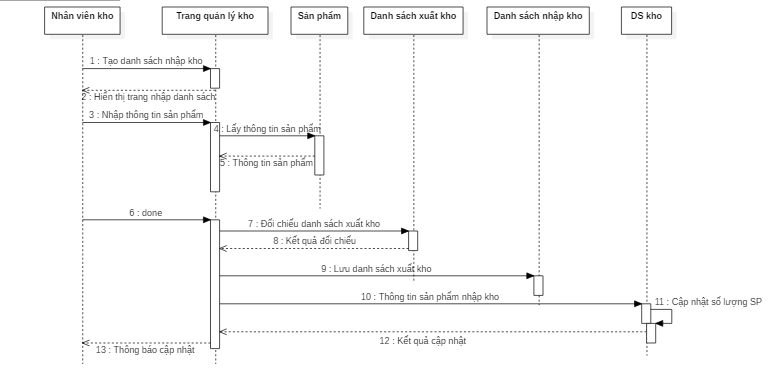
\includegraphics[scale = 0.5]{11.png}
        \caption{Biểu đồ Squence nhập kho}
    \end{figure}
    
\end{frame}

\begin{frame}{Sơ đồ nhập kho}
    \begin{figure}
        \centering
        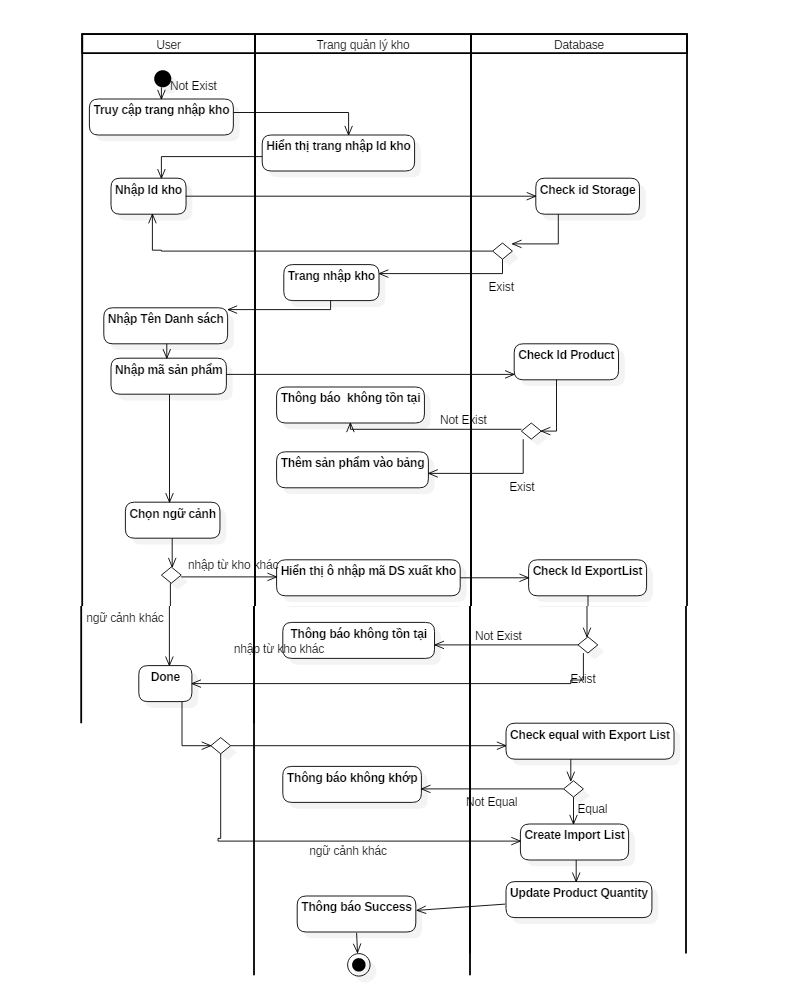
\includegraphics[scale  = 0.2]{35.png}
        \caption{Biểu đồ activity nhập kho}
    \end{figure}
\end{frame}


\begin{frame}{Chương 2.3: Qui trình quản lí kho - Thêm sản phẩm}
    \begin{itemize}
        \item Khi sản phẩm mới được nhập về thì sẽ chưa có dữ liệu trong hệ thống nên quản lí thực hiện việc tạo dữ liệu cho sản phẩm thông qua mã barcode.\\
        \item Khi tạo sản phẩm mới, từ dữ liệu barcode mà hãng đã cung cấp ta lấy được tên sản phẩm, size, Mã SP, màu sắc giá của sản phẩm sẽ do quản lý quy định và được nhập bởi quản lý hoặc nhân viên quản lý kho\\ 
        \item Sau khi đã điền đầy đủ các thông tin sản phẩm, nhân viên kho hoặc quản lý sẽ hoàn tất việc tạo dữ liệu cho sản phẩm mới. Hệ thống sẽ thêm dữ liệu sản phẩm vừa được tạo vào bảng Product .
    \end{itemize}
\end{frame}
\begin{frame}{Chương 2.3: Qui trình quản lí kho - Thêm sản phẩm}
    \begin{figure}
        \centering
        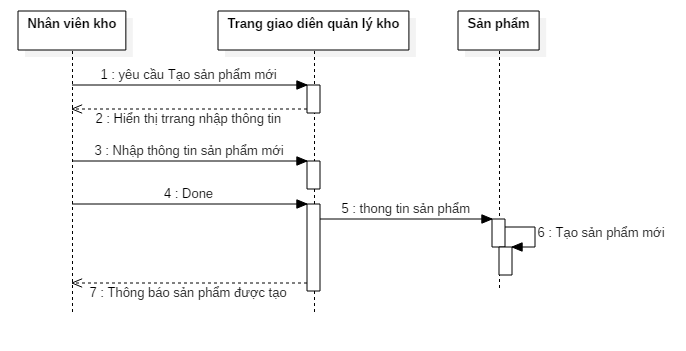
\includegraphics[scale =0.5]{12.png}

    \end{figure}
\end{frame}
\begin{frame}{Biểu đồ Class}
    \begin{figure}
        \centering
        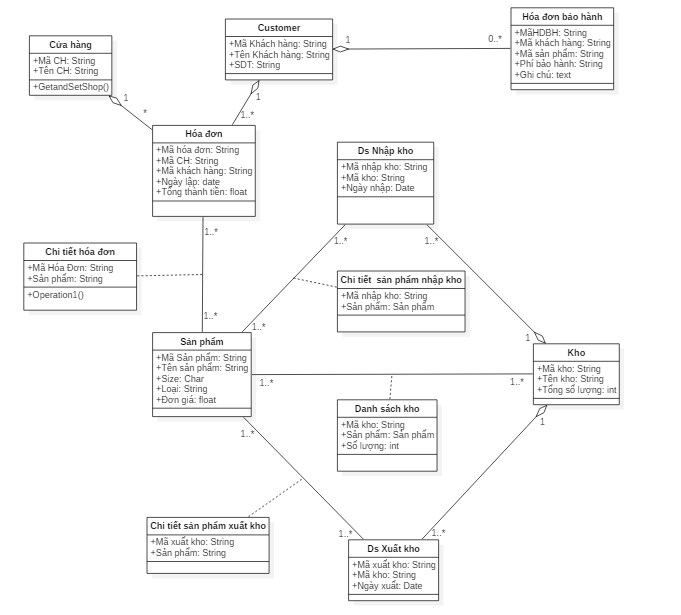
\includegraphics[scale = 0.5]{7.png}

    \end{figure}
\end{frame}


\begin{frame}{Biểu đồ ERD}
\begin{figure}
    \centering
    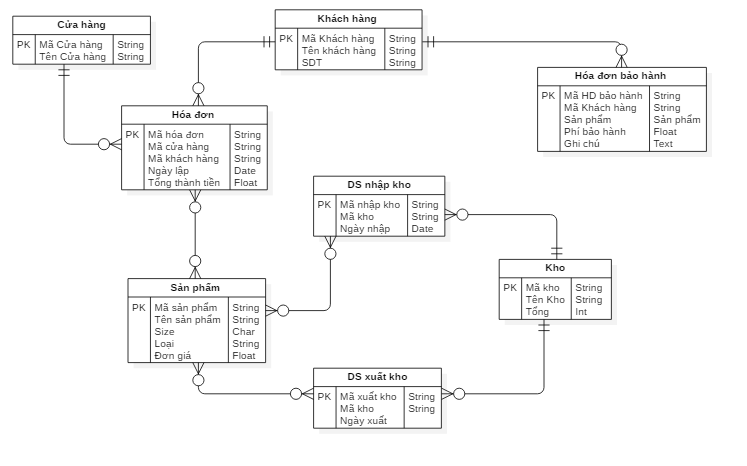
\includegraphics[scale = 0.5]{16.png}
    \caption{Biểu đồ ERD}
\end{figure}


\end{frame}



\end{document}

